\chapter{Introduction}
The focus of this mini project is to implement and optimise a piece of Python code. 
In this case the code snippet consists of two functions used in process of image processing of images of the iris. The functions are a noise remover function and a histogram equalisation function. In the following sections the functionalities of the functions are elaborated and the setup and approach for the optimisation is outlined. 

\section{The Functions}
\label{sec:The_Functions}
The images which are processed by the two functions are normalised images of the iris as can be seen in \autoref{fig:SimPolar}. First the image is handled by the noise remover function and then the output is handled by the Equalise histogram function. The following sections describe the functionalities of the functions. 
\begin{figure}[h]
\centering
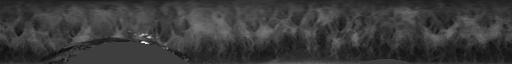
\includegraphics[width=\textwidth]{figures/002polar.jpg}
\caption{The normalised image of the iris before applying functions.}
\label{fig:SimPolar}
\end{figure}


\subsection{Noise Remover}
The purpose of the noise remover function is to remove noise occurring in the form of eyelashes covering parts of the iris. Usually the pixels showing the lashes will be among the darkest pixels. Since every image of the iris is different and how dark the iris is also varies, a threshold has to be identified adaptively. After the threshold has been found it is applied to all pixels in the image. If the pixels are lower than the threshold the pixels have to be eliminated and reconstructed from neighbouring pixels.
  
\subsection{Equalise Histogram}
This function has to identify the span of the "main" pixel values in the histogram. Once the "main" part of the  histogram has been identified this is stretched to cover the whole span of the range of the pixel values. This is done in order to increase the contrast in the image.  

